%% Начало содержательной части.
\chapter{Обзор предметной области}
В данной главе описаны основные определения из области поиска путей в теории графов. В первом разделе главы описаны понятия из теории графов. Во втором~-- из формальной области транспортных сетей. В третьем разделе формализуется задача и список требований по поддерживаемым свойствам для построения маршрутов. Четвертый раздел содержит краткое описание основных алгоритмов теории графов для поиска путей с описанием преимуществ и недостатков данных подходов.

\section{Основные определения}
\begin{definition}
Теория графов -- раздел дискретной математики, изучающий свойства графов.
\end{definition}

\begin{definition}
Граф -- это множество вершин (узлов), соединенных ребрами. В строгом определении графом называется такая пара множеств $G=\langle E, V \rangle$, где $V$ -- подмножество любого счетного множества, а $E$ -- подмножество $V \times V$.
\end{definition}

\begin{definition}
Маршрут -- это конечная последовательность вершин, в которой каждая вершина (кроме последней) соединена ребром со следующей в последовательности вершиной. Цепью называется маршрут без повторяющихся ребер. Простой цепью называется маршрут без повторяющихся вершин (откуда следует, что в простой цепи нет повторяющихся ребер).
\end{definition}

\begin{definition}
Ориентированный маршрут (или путь) -- это конечная последовательность вершин и дуг, в которой каждый элемент инцидентен предыдущему и последующему.
\end{definition}

\begin{definition}
Цикл -- это цепь, в которой первая и последняя вершины совпадают. При этом длиной пути (или цикла) называют число составляющих его ребер.
\end{definition}

\begin{definition}
Транспортное средство -- это совокупность технических систем, предназначенных для перемещений людей и грузов из одного места в другое.
\end{definition}

\begin{definition}
Транспортный узел -- это комплекс транспортных устройств в пункте стыка нескольких видов транспорта, совместно выполняющих операции по обслуживанию транзитных, местных и городских перевозок грузов и пассажиров.
\end{definition}

\begin{definition}
Транспортный рейс -- передвижение транспортного средства от места отправления до места назначения по заранее определённому маршруту и установленному расписанию, характеризуется выполнением определенной транспортной работы. В течение смены транспортное средство может осуществить несколько рейсов.
\end{definition}

\begin{definition}
Транспортная сеть -- это совокупность всех транспортных рейсов, представленных в течение интервала продажи билетов.
\end{definition}

\begin{definition}
Остановка -- специально отведенное общественное место, предназначенное для посадки/высадки пассажиров рейсового транспортного средства.
\end{definition}

\begin{definition}
Расписание -- таблица, для которой указана информация о предстоящих (планируемых или потом произошедших) событиях.
\end{definition}

\begin{definition}
Мульмодальный маршрут -- это конечная последовательность транспортных рейсов, попав на которые в определенные промежутки времени можно добраться от начального транспортного узла до конечного.
\end{definition}

\begin{definition}
Построитель маршрутов -- это программный комплекс для обработки внешних поисковых клиентских запросов, имеющий доступ к полному объему данных о расписаниях на всех транспортных узлах и осуществляющий выдачу определенного количества маршрутов в соответствии с поступившими в запросах требованиями. Также в качестве дополнительных возможностей доступно построение фильтров и различной статистики (активные транспортные узлы, активные транспортные рейсы, проходящие через заданный узел).
\end{definition}

\begin{definition}
Клиентское приложение -- это любое приложение, которое осуществляет запросы к построителю маршрутов за результатом (маршрутами и фильтрами).
\end{definition}

\section{Виды транспорта и его особенности}
В транспортной сети, в которой будут строиться маршруты, будет существовать только транспорт с конкретным расписанием транспортных рейсов. Таким образом, идет допущение о том, что система сети идеальна и весь транспорт гарантировано совершает остановки в назначенное время. Постановка вспомогательных свойств для построителя маршрутов, которые позволяют сгладить последствия этого допущения, будут описаны в следующих главах. Далее рассмотрим виды транспорта.

\subsection{Железнодорожный}
В задаче будут использоваться 2 вида железнодорожного транспорта. Во-первых, это будут поезда дальнего следования, у которых небольшое количество рейсов (около $10^5$ в течение интервала продажи билетов). Во-вторых, это будут электрички, которые уже совершают до $10^6$ рейсов за аналогичный промежуток времени.
Транспортными узлами являются железнодорожные станции и вокзалы.

\subsection{Воздушный}
Воздушный транспорт будет представлен только самолетами. При этом количество рейсов около $10^3$, поэтому особый интерес этот случай не представляет. Но стоит отметить, что в большинстве случаев мультимодальный маршрут не будет содержать больше одного воздушного сегмента пути.
Транспортными узлами являются аэропорты.

\subsection{Автомобильный}
Автомобильный транспорт состоит из автобусных междугородних рейсов. Около 95\% таких рейсов совершаются только между соседними городами, что сильно упрощает задачу, но их количество все равно большое~—~$10^6$.
Также в эту категорию входит транспорт в пределах города (или любого крупного населенного пункта), например, такси. Стоит отметить, что в этот вид транспорта можно внести любые другие средства передвижения внутри города, так как в конечном счете это не будет влиять на алгоритм. При этом важно, чтобы у нового транспорта в пределах города имелась возможность рассчитать эвристическое времени передвижения между двумя транспортными узлами, которые относятся к одному населенному пункту. Эту задачу следует решать на основе статистики или с помощью сторонних сервисов, которые умеют анализировать дорожную ситуацию и могут оценить время движения на основе карты автомобильных заторов.
Транспортными узлами являются автобусные остановки и крупные населенные пункты.

\section{Построение маршрутов}
Основная задача, ставящаяся перед построителем маршрутов — построение маршрутов по данным в его памяти и внешних базах данных, доступных для чтения в конкретный момент времени. На алгоритм построения маршрутов в транспортной сети накладываются следующие условия и ограничения.

\subsection{Мультимодальность}
Маршруты могут быть мультимодальными, то есть проходить через несколько точек-остановок, содержать пересадки, проходить разными видами транспорта со своими особенностями и т.д.; Это нужно для того, чтобы была возможность добраться из любой точки в любую, где есть хотя бы какой-нибудь транспорт. Вариант пройти пешком небольшой кусок пути тоже доступен внутри крупного населенного пункта.
\begin{figure}[!h]
    \centering
    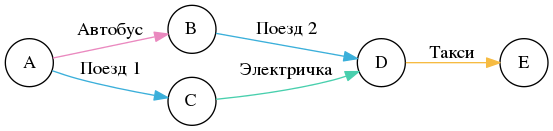
\includegraphics[width=0.9\textwidth]{multimodal_example.png}
    \caption{Несколько мультимодальных маршрутов от точки A до точки E.}\label{fig1}
\end{figure}

\subsection{Временные интервалы}
Маршруты можно строить для определенных интервалов времени. Например, хотим выехать в промежуток с 8-00 до 12-00 утра, а приехать в любой день на следующей неделе, но обязательно после 21-00. Это требуется для того, чтобы иметь возможность бронировать гостиницу, не отходя от кассы.

\subsection{Инкрементальное построение}
Маршруты требуется строить инкрементально (не все сразу, а только небольшую часть из существующих) из-за того, что возможное количество маршрутов может достигать до $10^9$ между парой крупных населенных пунктов с 3 допустимыми пересадками и интервалом времени в пути равным нескольким дням. Это требуется для конечного клиентского приложения, чтобы можно было организовать страничный показ результатов без полного вычисления всех маршрутов на предыдущих страницах.

\subsection{Адаптивность}
Маршруты могут строиться адаптивно по времени из-за того, что важно время отклика алгоритма, то есть в приоритете время выполнения над показом действительно всех требуемых результатов.

\section{Построение фильтров к доступным маршрутам}
Под фильтром в данном случае понимается предикат, который принимает в качестве аргумента построенный маршрут и возвращает ИСТИНА или ЛОЖЬ в зависимости от того, удовлетворяет ли маршрут критериям поиска, которые задает фильтр.
Таким образом, помимо построения самих маршрутов, требуется построить фильтры по доступным маршрутам с условиями, перечисленными далее.

\subsection{Косвенные признаки}
Из-за того, что маршруты строятся не все сразу, то кроме непосредственно найденных маршрутов существует огромное количество потенциально доступных маршрутов. При этом мы хотим получить к ним доступ по косвенным признаками. Например, это может быть тип транспорта, номер поезда или тип места в самолете (у окна/у туалета/в хвосте). Формально любой параметр доступный в модели данных может стать доступным для фильтрации\footnote{Под моделью данных в данном случае подразумевается любой абстрактный объект, который имеет отражение в реальном мире: поезд, самолет, аэропорт и т.д.}.

\subsection{Осуществление фильтрации}
Фильтрацию мы хотим осуществлять как можно раньше для некоторых фильтров, и позже -- для других, потому что некоторые проверки могу занять большое количество времени. Дополнительно мы хотим поддерживать несколько типов фильтрации:
\begin{itemize}
	\item \textbf{Фильтрация по отрезкам}. Переданный фильтр должен пропускать каждый сегмент маршрута. При этом для каждого типа косвенного признака может быть задан один из нескольких предикатов.
	\item \textbf{Фильтрация по маршрутам}. В данном случае фильтр должен пропускать маршрут целиком. Примером такого фильтра может быть количество свободных мест.
	\item \textbf{Дополнительные условия}. В эту категорию входят особые фильтры бизнес-логики, они не задаются специально через клиентское приложение, но действуют для всех найденных маршрутов. Примером таких фильтров служит то, что в маршруте не должны повторяться станции или рейсы.
\end{itemize}

\subsection{Функциональные зависимости}
Не последнюю роль в фильтрах играют функциональные зависимости, потому что в последствии фильтры нужно будет удобно отображать без противоречий в клиентском приложении. Например, тип места «у окна» в купе и каюте относятся к разным типам транспорта и их нельзя объединять. Пример «дерева» функциональный зависимостей для поезда:
\begin{itemize}
    \item Точки отправления и прибытия
    \item Интервалы отправления и прибытия
	\item Вид транспорта - Поезд:
	\begin{itemize}
		\item Перевозчик
		\item Бренд
		\item Номер
		\item Тип вагона:
		\begin{itemize}
			\item Купе:
			\begin{itemize}
				\item Верхнее/нижнее
				\item Не у туалета
			\end{itemize}
			\item Сидячий:
			\begin{itemize}
				\item У окна/у прохода
			\end{itemize}
			\item Плацкарт:
			\begin{itemize}
				\item Верхнее/нижнее
				\item Не у туалета
				\item Боковое/не боковое
			\end{itemize}
		\end{itemize}
	\end{itemize}
\end{itemize}

Каждый уровень списка зависит от родительского уровня и строго им определяется для того, чтобы исключить ситуации, когда несколько косвенных признаков совпадают у разных видов транспорта. Например, признак «Перевозчик» у поезда и самолета. Такое разделение необходимо для корректного с точки зрения логики и удобного вывода результата в клиентском приложении.

\section{Сортировка маршрутов}
Маршруты требуется строить в порядке сортировки. В простейшем варианте можно сортировать только построенные маршруты, что не представляет из себя никакой сложности. В сложном варианте маршруты строятся на основе любого предиката сравнения пары маршрутов и выдаются в результат, гарантируя определенный порядок. В рамках данной работы подходит «средний» вариант. Требуется гарантировать определенный порядок построенных маршрутов без пропусков, но предикаты известны заранее. Всего их 4 основных вида:
\begin{enumerate}
    \item Количество пересадок;
    \item Время отправления;
    \item Время прибытия;
    \item Время в пути;
\end{enumerate}

Далее рассмотрим некоторые из них более подробно.

\subsection{Количество пересадок}
Самая простая сортировка в рамках данной работы (или просто сортировка по-умолчанию). Несложно заметить, что количество пересадок будет пропорционально количеству транспорта, который включен в мультимодальный маршрут. И если представить каждый отрезок пути на конкретном транспорте отдельным ребром в абстрактном графе, то сортировка будет происходить относительно количества ребер.

\subsection{Время отправления/прибытия}
У каждой остановки любого транспортного рейса существует время прибытия и время отбытия. У первой и последней остановок оно совпадает. Если задан бесконечный или полу-бесконечный интервал, то нижний предел времени ограничен текущим серверным временем, а верхний предел -- неким разумным пределом, например, датой продаж. Для выбора верхней границы существуют разные стратегии. Например, при заданном интервале отправления можно устанавливать интервал прибытия зависимым от него. Для этого нужно знать максимальную продолжительность пути в системе, что не представляет сложности при ограничении максимального количества пересадок.

\section{Известные алгоритмы}
В этом разделе мы рассмотрим типовые алгоритмы для поиска маршрутов в графе. Многие известные сервисы для заказа билетов работают на их основе с некоторыми дополнениями для поддержания требуемой бизнес-логики.
\subsection{Алгоритм Дейкстры}
Классический алгоритм для вычисления кратчайших путей в статическом графе $G=(V, E)$ с функцией веса\footnote{Предполагается, что в статическом графе ребра имеют неотрицательные веса. Для общего случая можно использовать алгоритм Беллмана — Форда.} для ребер называется алгоритмом Дейкстры. В частности, алгоритм, разработанный Э. Дейкстрой, решает проблему нахождения кратчайших маршрутов от единственной стартовой вершины $s$ до всех остальных вершин в графе $G$. Алгоритм поддерживает для каждой вершины $u$ метку $\delta(u)$ с предварительным расстоянием от $s$ до $u$. Каждая вершина может находиться в одном из следующих состояний: нерассмотренная, рассмотренная, посещенная. 

\begin{algorithm}[!h]
	\caption{Алгоритм Дейкстры}\label{lst1}
	\begin{algorithmic}
		\Function{Dijkstra}{$s$}
		\State $\delta = \left\{\infty, ..., \infty\right\}$ \Comment{предварительные расстояния}
		\State $\delta(s) = 0$ \Comment{поиск начинается из вершины $s$}
		\State $Q.update(0, s)$ \Comment{приоритетная очередь}
		\While{$Q \neq \emptyset $}
		\State $(\_, u)$ = Q.deleteMin() \Comment{посещаем $u$}
		\For{$ e = (u, v) \in E$} \Comment{релаксируем ребра}
		\If{$ \delta(u) + c(e) < \delta(v) $}
		\State $delta(v) = \delta(u) + c(e)$
		\State $Q.update(\delta(v), v)$
		\EndIf
		\EndFor
		\EndWhile
		\EndFunction
	\end{algorithmic}
\end{algorithm}

Изначально только вершина $s$ считается рассмотренной с $\delta(s)=0$ и все остальные вершины $u$ являются нерассмотренными с $\delta(u)=\infty$.

На каждом шаге вершина $u$ с минимальной $\delta(u)$ извлекается и удаляется из приоритетной очереди $Q$. Будем говорить, что вершина посещена, так как теперь известно, что $\delta(u)$ -- кратчайшее расстояние. Все исходящие ребра $(u, v)$ посещенной вершины релаксируются, то есть сравнивается кратчайшее расстояние от $s$ через $u$ до вершины $v$ с предварительным расстоянием $\delta(v)$. Если оно меньше, то мы обновляем $\delta(v)$ и $v$ в приоритетной очереди $Q$. Стоит заметить, что такое обновление для нее это либо операции вставки, если вершина рассмотрена, либо операция уменьшения ключа в противном случае. Алгоритм заканчивает работу только тогда, когда очередь становится пустой. Это произойдет после $n$ шагов, где $n$ -- это количество вершин в графе $G$.

В приведенном псевдокоде видно, что иногда мы не посещаем все вершины в графе. Это происходит из-за того, что либо такие вершины недостижимы из $s$, либо очередь становится пустой раньше, чем мы доходим до такой вершины. Для того, чтобы избежать инициализации алгоритма за $O(n)$ при последовательных вызовах, можно сохранять посещенные вершины и обновлять их значения $\delta$ после конца алгоритма. Таким образом, асимптотика алгоритма зависит только от количества посещенных вершин и релаксируемых ребер, а не от $n$. 

Алгоритм Дейкстры использует максимум $n$ операций вставки в приоритетную очередь, $n$ удалений и $m$ операций уменьшения ключа, обеспечивая таким образом асимптотику $O(m + n \log n)$ при использовании Фибоначчиевой кучи.

\begin{figure}[!h]
	\centering
	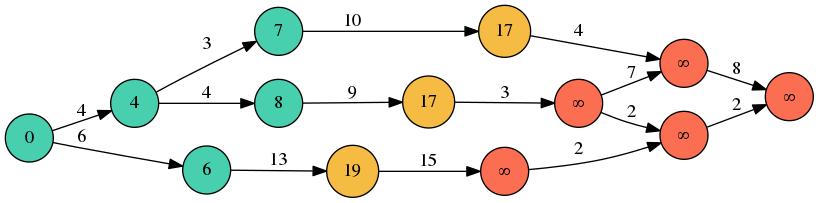
\includegraphics[width=\textwidth]{dijkstra_example.png}
	\caption{Состояние алгоритма Дейкстры после посещения 5 вершин. Посещенные - зеленые, рассмотренные - желтые, нерассмотренные - красные.}\label{fig1}
\end{figure}

\FloatBarrier
\subsection{Алгоритм Йена}
Алгоритм Йена находит $k$ путей без циклов от единственной стартовой вершины $s$ до конечной вершины $t$ в статичном графе. Разработанный Йеном алгоритм предполагает, что в его основе будет лежать любой другой алгоритм поиска кратчайшего пути, например, его основой может послужить алгоритм Дейкстры. Идея основана на том, что можно построить изначально кратчайший путь и потом на основе этого пути искать ответвления, чтобы построить следующий. Каждая $k$ итерация будет искать ответвления от кратчайших путей, полученных на $k-1$ итерациях.
\begin{algorithm}[!h]
	\caption{Алгоритм Йена}\label{lst2}
	\begin{algorithmic}
		\Function{Yen}{$s$, $t$, $K$}
		\State $A[0] = Dijkstra(s, t)$ \Comment{определяем кратчайший путь от $s$ до $t$}
		\State $B = \emptyset$ \Comment{приоритетная очередь, хранящая кандидатов на $k$ кратчайший путь}
		\For{$k = 1$ to $K$}
			\For{$i = 0$ to $size(A[k-1]) - 1] $}
				\State $spurNode = A[k-1].node(i)$ \Comment{Вершина ответвления извлекается из полученного на предыдущей итерации пути}
				\State $rootPath = A[k-1].nodes(0, i)$ \Comment{Последовательность вершин от стартовой до вершины ответвления образуют корневой префикс пути}
				
				\For{$p \in A$}
					\If{$rootPath = p.nodes(0,i)$}
						\State удаляем $p.edge(i, i+1)$ из графа
					\EndIf
				\EndFor
				
				\For{$rootPathNode \in rootPath$}
					\If{$rootPathNode \neq spurNode$}
						\State удаляем $rootPathNode$ из графа
					\EndIf
				\EndFor
				
				\State $spurPath = Dijkstra(spurNode, t)$ \Comment{вычисляем путь-ответвление}
				
				\State $totalPath = rootPath + spurPath$ \Comment{Полный путь состоит из корневого префикса и пути-ответвления}
				\State $B.append(totalPath)$ \Comment{Добавление кандидата на кратчаший $k$ путь}
				
				\State восстанавливаем в графе удаленные на текущей итерации ребра и вершины
			\EndFor
			
			\If{$B = \emptyset$}
				\State \textbf{break}
			\EndIf
			\State $(\_, A[k]) = B.deleteMin()$
		\EndFor
		\EndFunction
	\end{algorithmic}
\end{algorithm}

\chapterconclusion
В главе были обозначены цели и задачи: поиск маршрутов в соответствии с правильной сортировкой и получение фильтров для доступных маршрутов по заданному запросу. Также были показаны подходы для поиска.